\documentclass[nohyper,justified]{tufte-handout}\usepackage{graphicx, color}
%% maxwidth is the original width if it is less than linewidth
%% otherwise use linewidth (to make sure the graphics do not exceed the margin)
\makeatletter
\def\maxwidth{ %
  \ifdim\Gin@nat@width>\linewidth
    \linewidth
  \else
    \Gin@nat@width
  \fi
}
\makeatother

\definecolor{fgcolor}{rgb}{0.2, 0.2, 0.2}
\newcommand{\hlnumber}[1]{\textcolor[rgb]{0,0,0}{#1}}%
\newcommand{\hlfunctioncall}[1]{\textcolor[rgb]{0.501960784313725,0,0.329411764705882}{\textbf{#1}}}%
\newcommand{\hlstring}[1]{\textcolor[rgb]{0.6,0.6,1}{#1}}%
\newcommand{\hlkeyword}[1]{\textcolor[rgb]{0,0,0}{\textbf{#1}}}%
\newcommand{\hlargument}[1]{\textcolor[rgb]{0.690196078431373,0.250980392156863,0.0196078431372549}{#1}}%
\newcommand{\hlcomment}[1]{\textcolor[rgb]{0.180392156862745,0.6,0.341176470588235}{#1}}%
\newcommand{\hlroxygencomment}[1]{\textcolor[rgb]{0.43921568627451,0.47843137254902,0.701960784313725}{#1}}%
\newcommand{\hlformalargs}[1]{\textcolor[rgb]{0.690196078431373,0.250980392156863,0.0196078431372549}{#1}}%
\newcommand{\hleqformalargs}[1]{\textcolor[rgb]{0.690196078431373,0.250980392156863,0.0196078431372549}{#1}}%
\newcommand{\hlassignement}[1]{\textcolor[rgb]{0,0,0}{\textbf{#1}}}%
\newcommand{\hlpackage}[1]{\textcolor[rgb]{0.588235294117647,0.709803921568627,0.145098039215686}{#1}}%
\newcommand{\hlslot}[1]{\textit{#1}}%
\newcommand{\hlsymbol}[1]{\textcolor[rgb]{0,0,0}{#1}}%
\newcommand{\hlprompt}[1]{\textcolor[rgb]{0.2,0.2,0.2}{#1}}%

\usepackage{framed}
\makeatletter
\newenvironment{kframe}{%
 \def\at@end@of@kframe{}%
 \ifinner\ifhmode%
  \def\at@end@of@kframe{\end{minipage}}%
  \begin{minipage}{\columnwidth}%
 \fi\fi%
 \def\FrameCommand##1{\hskip\@totalleftmargin \hskip-\fboxsep
 \colorbox{shadecolor}{##1}\hskip-\fboxsep
     % There is no \\@totalrightmargin, so:
     \hskip-\linewidth \hskip-\@totalleftmargin \hskip\columnwidth}%
 \MakeFramed {\advance\hsize-\width
   \@totalleftmargin\z@ \linewidth\hsize
   \@setminipage}}%
 {\par\unskip\endMakeFramed%
 \at@end@of@kframe}
\makeatother

\definecolor{shadecolor}{rgb}{.97, .97, .97}
\definecolor{messagecolor}{rgb}{0, 0, 0}
\definecolor{warningcolor}{rgb}{1, 0, 1}
\definecolor{errorcolor}{rgb}{1, 0, 0}
\newenvironment{knitrout}{}{} % an empty environment to be redefined in TeX

\usepackage{alltt}
%\documentclass{article}
%\usepackage[absolute,showboxes]{textpos}
\usepackage[absolute]{textpos}
\usepackage{sidecap}
%\usepackage{color}
%\usepackage[usenames,dvipsnames,svgnames,table]{xcolor}
\IfFileExists{upquote.sty}{\usepackage{upquote}}{}
\begin{document}
 



\begin{wide}
\section{\Huge Porfolio Report: 080512_2 4x b }

\hrulefill 
\end{wide}

\begin{textblock*}{105mm}(105mm,40mm)
\begin{figure}
\vspace{0pt}
\begin{knitrout}
\definecolor{shadecolor}{rgb}{0.969, 0.969, 0.969}\color{fgcolor}
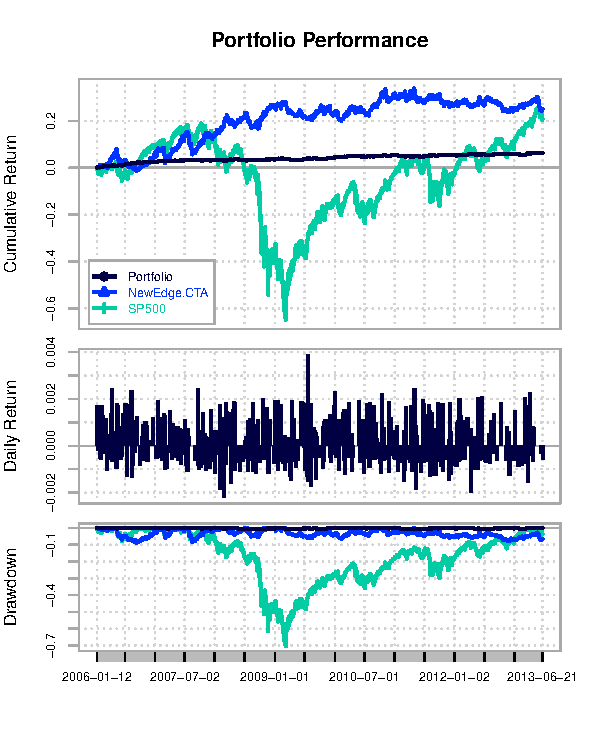
\includegraphics[width=\maxwidth]{figure/Performance} 

\end{knitrout}

\end{figure}
\end{textblock*}

% \begin{textblock*}{95mm}(10mm,134mm)
% \begin{figure}
% \vspace{0pt}
% <<Performance2,echo=FALSE,eval=TRUE,fig.width=8,fig.height=3>>=
% pnl.monthly <- period.apply(ptf.daily[,1],INDEX=endpoints(ptf.daily,'months'),FUN=sum)
% barplot(pnl.monthly*100,main="Monthly Returns (% AUM)")
% @
% \end{figure}
% \end{textblock*}


\begin{textblock*}{75mm}(15mm,50mm)
\Large Summary Statistics
\normalsize
%\newline
\begin{figure}
\vspace{0pt}
% latex table generated in R 2.15.2 by xtable 1.7-1 package
% Thu Aug 29 14:06:22 2013
\scalebox{0.7}{
\begin{tabular}{lrrr}
  \hline
 & Portfolio & NewEdge.CTA & SP500 \\ 
  \hline
Total Return (\% AUM) & 6.34 & 24.89 & 20.74 \\ 
  Compounded Annual Return (\%) & 0.82 & 3.01 & 0.16 \\ 
  Max Drawdown (\% AUM) & 0.87 & 9.94 & 61.03 \\ 
  Days to Recovery & 88.00 & 88.00 & 88.00 \\ 
  Annualized Volatility (\%) & 0.84 & 7.21 & 22.47 \\ 
  Correlation with SP500 (\%) & 100.00 & -0.42 & 2.17 \\ 
  Sharpe Ratio & 0.98 & 0.42 & 0.01 \\ 
  Sortino Ratio & 0.11 & 0.04 & 0.01 \\ 
  Skewness & 1.32 & -0.53 & -0.30 \\ 
  Kurtosis & 9.12 & 5.28 & 12.42 \\ 
  Omega Ratio & 1.29 & 1.08 & 1.02 \\ 
  Kelly Fraction & 58.86 & 3.10 & 0.27 \\ 
  Total Return since 1 Jan 2010 (\% AUM) & 1.99 & 2.45 & 35.63 \\ 
  Total Return since 1 Jan 2011 (\% AUM) & 0.92 & -6.66 & 23.60 \\ 
  Total Return since 1 Jan 2012 (\% AUM) & 0.98 & -2.32 & 23.61 \\ 
  Total Return since 1 Jan 2013 (\% AUM) & 0.63 & 0.38 & 11.03 \\ 
   \hline
\end{tabular}
}


\end{figure}

\vspace{5mm}
\small Drawdown Length and Recovery Times
\normalsize
\begin{figure}
% latex table generated in R 2.15.2 by xtable 1.7-1 package
% Thu Aug 29 14:06:22 2013
\scalebox{0.7}{
\begin{tabular}{rlllrr}
  \hline
 & Start & Trough & Recovery & Max Drawdn (\%) & Duration \\ 
  \hline
1 & 2010-12-30 & 2011-06-15 & 2011-10-17 & -0.87 & 208 \\ 
  2 & 2009-02-17 & 2009-04-14 & 2009-07-23 & -0.83 & 113 \\ 
  3 & 2008-05-01 & 2008-07-15 & 2009-01-22 & -0.81 & 191 \\ 
  4 & 2009-07-24 & 2009-10-22 & 2009-12-29 & -0.66 & 113 \\ 
  5 & 2012-04-12 & 2013-03-07 & 2013-03-20 & -0.64 & 245 \\ 
   \hline
\end{tabular}
}


\end{figure}
\end{textblock*}


\begin{textblock*}{180mm}(15mm,160mm)
\begin{figure}
\vspace{0pt}
\begin{knitrout}
\definecolor{shadecolor}{rgb}{0.969, 0.969, 0.969}\color{fgcolor}
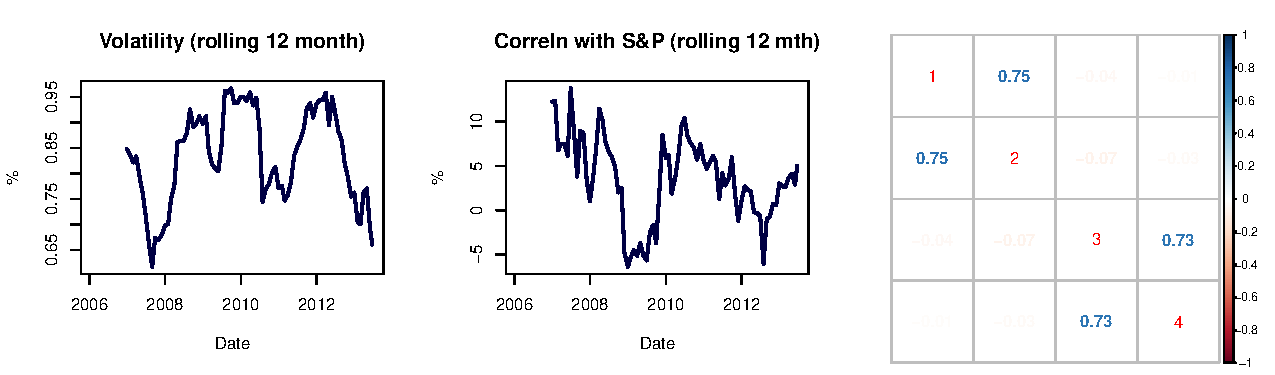
\includegraphics[width=\maxwidth]{figure/voletc} 

\end{knitrout}

\end{figure}
\end{textblock*}

% \begin{textblock*}{180mm}(15mm,170mm)
% \begin{figure}
% \vspace{0pt}
% <<cortable,echo=FALSE,warning=TRUE,eval=TRUE>>=
% 
% print(xtable(cor(rtns.xts),digits=3),floating=FALSE, scalebox=0.7)
% @
% \end{figure}
% \end{textblock*}

\begin{textblock*}{180mm}(15mm,210mm)
\begin{figure}
\vspace{0pt}
\begin{knitrout}
\definecolor{shadecolor}{rgb}{0.969, 0.969, 0.969}\color{fgcolor}
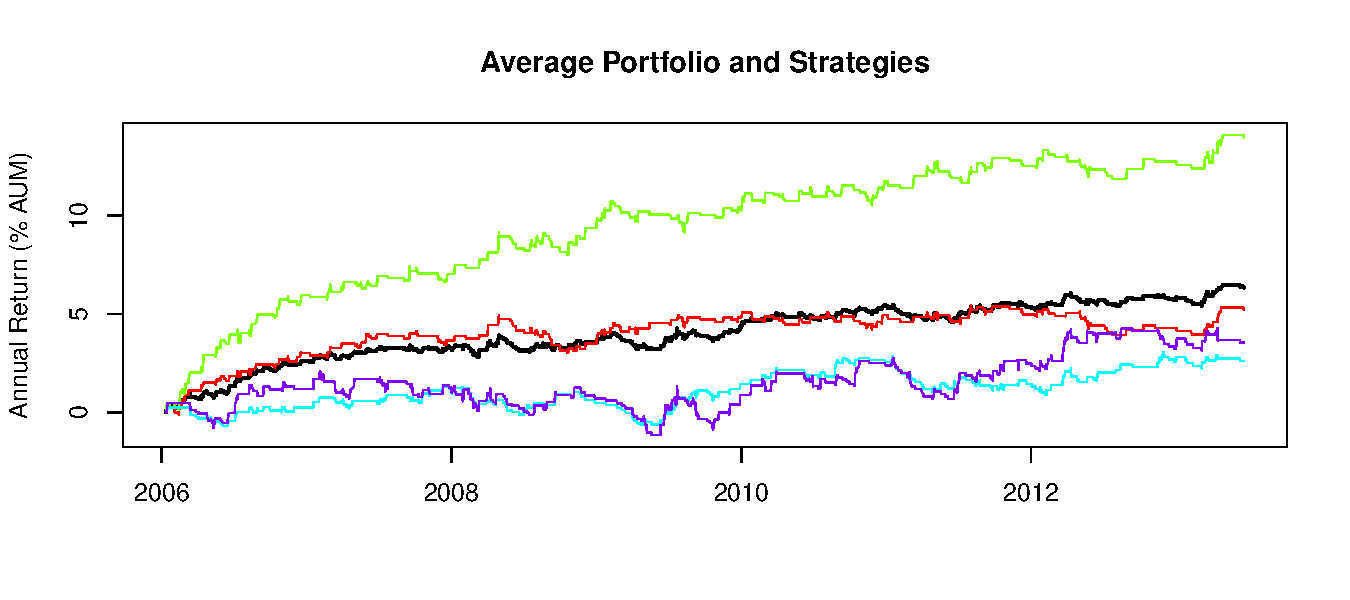
\includegraphics[width=\maxwidth]{figure/Performance2} 

\end{knitrout}

\end{figure}
\end{textblock*}


\end{document}
